% Technique Titan — technical report (Overleaf / pdfLaTeX)
% Compiler: pdfLaTeX. No extra files required.
\documentclass[11pt,a4paper]{article}

\usepackage[margin=1in]{geometry}
\usepackage[T1]{fontenc}
\usepackage[utf8]{inputenc}
\usepackage{lmodern}
\usepackage{microtype}
\usepackage{setspace}
\usepackage{amsmath,amssymb,amsthm}
\usepackage{booktabs}
\usepackage{tabularx}
\usepackage{array}
\usepackage{longtable}
\usepackage{enumitem}
\usepackage{xcolor}
\usepackage{tikz}
\usetikzlibrary{arrows.meta,positioning,calc,fit,shapes.geometric,decorations.pathreplacing}
\usepackage{graphicx}
\usepackage{caption}
\usepackage{subcaption}
\usepackage{fancyhdr}
\usepackage{titlesec}
\usepackage{xurl}
\usepackage{hyperref}
\usepackage{csquotes}
\usepackage{parskip}

\onehalfspacing
\setlist[itemize]{leftmargin=1.4em,itemsep=0.25em,topsep=0.4em}
\setlist[enumerate]{leftmargin=1.6em,itemsep=0.25em,topsep=0.4em}

\definecolor{ttink}{HTML}{1A1A1A}
\definecolor{ttaccent}{HTML}{2F6FED}
\definecolor{ttgood}{HTML}{2E7D32}
\definecolor{ttwarn}{HTML}{E65100}
\definecolor{ttcrit}{HTML}{C62828}
\definecolor{ttgray}{HTML}{555555}

\hypersetup{
  colorlinks=true,
  linkcolor=ttaccent,
  citecolor=ttaccent,
  urlcolor=ttaccent,
  pdftitle={Technique Titan: Building an AI Piano Posture Coach},
  pdfauthor={Aaron Dutta}
}

\titleformat{\section}{\large\bfseries\raggedright}{\thesection}{0.8em}{}
\titleformat{\subsection}{\normalsize\bfseries\raggedright}{\thesubsection}{0.7em}{}
\titleformat{\subsubsection}{\normalsize\itshape\raggedright}{\thesubsubsection}{0.7em}{}

\pagestyle{fancy}
\fancyhf{}
\fancyhead[L]{\small\textit{Technique Titan}}
\fancyhead[R]{\small Aaron Dutta}
\fancyfoot[C]{\thepage}
\renewcommand{\headrulewidth}{0.3pt}

\newcommand{\tturl}[1]{\url{#1}}
\newcommand{\code}[1]{\texttt{#1}}

\begin{document}

\begin{titlepage}
\centering
\vspace*{1.4cm}
{\Large\bfseries Technique Titan}\\[0.45cm]
{\LARGE Building an AI Piano Posture Coach}\\[0.7cm]
{\large From a MediaPipe prototype to a deployed detect--score--coach product}\\[1.4cm]
{\large Aaron Dutta}\\[0.35cm]
{\normalsize Honours Mathematics, University of Waterloo}\\[0.15cm]
{\normalsize Pianist, Royal Conservatory of Music Level~10 with Honours}\\[1.1cm]
{\normalsize A technical report on the concepts, architecture, timeline,}\\[0.1cm]
{\normalsize and integration of the Technique Titan system}\\[1.4cm]
{\normalsize September 2026}\\[0.3cm]
{\small Live product: \tturl{https://technique-titan.vercel.app}}\\[0.15cm]
{\small Source: \tturl{https://github.com/defAaron/TechniqueTitan}}\\[2.2cm]
\begin{minipage}{0.88\textwidth}
\small
\noindent\textit{Abstract.}
Technique Titan is an AI piano posture coach that turns a laptop or phone camera into on-demand technique feedback.
It detects twenty-one MediaPipe landmarks per hand, normalizes them so measurements are invariant to camera distance and hand size, computes five geometric criteria drawn from piano pedagogy, maps those metrics onto 0--100 scores and severity bands, and returns prioritized plain-language coaching.
This report is the story of how that system was built: the pedagogical problem, the computer-vision and geometry ideas underneath it, the software architecture that grew around a shared Python engine, the timeline from a 2024 hand-tracking sketch to a 2026 React and FastAPI product with evaluation and offline machine learning, and the way those pieces now fit together.
Production scoring remains explainable YAML heuristics; a logistic-regression scorer exists offline and is not yet on the serving path.
\end{minipage}
\vfill
\end{titlepage}

\tableofcontents
\newpage

%----------------------------------------------------------------------
\section{Introduction}
%----------------------------------------------------------------------

Most of a pianist's hours happen alone.
A teacher might see a student once a week.
In the hours between lessons, collapsed wrists, flat fingers, and tucked thumbs become muscle memory.
The feedback that would stop those habits is usually qualitative---\enquote{rounder fingers}, \enquote{don't drop the wrist}---and it arrives too infrequently to compete with repetition.

I built Technique Titan to close that loop.
The product uses a standard RGB camera.
It does not require gloves, depth sensors, or a motion-capture lab.
For each visible hand it extracts a 21-point skeleton, measures five posture criteria that piano teachers already talk about, scores each criterion on a 0--100 scale, and returns the one coaching tip that matters most right now.

This is not a note-correctness app and not a medical device.
It evaluates \emph{posture}: wrist height, finger curvature, thumb position, wrist lateral deviation, and overall hand arch.
Musical accuracy---notes, rhythm, dynamics---is explicitly out of scope.

The project sits at the intersection of two lives I actually live.
I have played piano for fourteen years, including Royal Conservatory of Music Level~10 with Honours.
I am a first-year Honours Mathematics student at the University of Waterloo.
Technique Titan is the place those two practices meet: the musician who knows how fragile healthy technique is, and the builder who wanted objective, repeatable measurement instead of another untestable slogan.

This report has three jobs.
First, it explains the \emph{concepts}: MediaPipe Hands, coordinate normalization, joint angles, plane fitting, piecewise-linear scoring, templated coaching, hold-out evaluation, and multinomial logistic regression.
Second, it reconstructs the \emph{journey}: what existed in 2024, what was rebuilt in the summer of 2026, which product surfaces shipped in which month, and which production failures forced architectural decisions.
Third, it shows how the pieces \emph{come together} today: a shared Python library behind a batch CLI, a Streamlit research UI, a FastAPI backend, a React product on Vercel, optional Supabase accounts, a Notion labeling table, and an offline ML loop that is deliberately not yet production.

The live site is \tturl{https://technique-titan.vercel.app};
the API is \tturl{https://technique-titan-api.onrender.com}.
The source of truth for requirements is the in-repo product requirements document~\cite{prd}; the delivery plan is the roadmap~\cite{roadmap}.

%----------------------------------------------------------------------
\section{The problem Technique Titan is trying to solve}
%----------------------------------------------------------------------

\subsection{Why piano posture is hard to coach at scale}

Healthy piano technique is a small-geometry problem.
A wrist that sits level with the knuckle line, fingers that hold a soft curve as if around a bubble, a thumb that rests on its side rather than tucking under or flaring out, a forearm-to-hand line that is not bent hard toward the pinky or the thumb, and a knuckle bridge that forms a gentle dome: these are the shapes teachers correct in the studio.
They decide tone, speed, endurance, and comfort.
They also drift quietly.
A dropped wrist feels normal after a few days.
By the time it hurts, or a teacher catches it, the motion is already practiced.

Three structural gaps make this worse than it needs to be.

\begin{enumerate}
  \item \textbf{Infrequent feedback.} Students practice far more hours than they spend with a teacher, so habits form in the gap.
  \item \textbf{No objective measurement.} \enquote{Rounder fingers} is hard for a beginner to internalize or track across weeks.
  \item \textbf{Uneven access.} Self-taught learners and remote students often get no posture feedback at all. Mirrors and phone recordings only help if you already know what to look for, and you cannot watch your own hands while you play.
\end{enumerate}

Technique Titan's bet is that a camera plus geometry can provide \emph{objective, repeatable, on-demand} evaluation without specialized hardware.
That is a different bet from \enquote{train a giant vision model on pixels and hope it agrees with a teacher.}
The product is designed to stay explainable: every score traces back to a named landmark measurement~\cite{scoringmethods}.

\subsection{Personas and use cases}

The product requirements document names four personas: a self-taught beginner, a student of a teacher, a piano teacher reviewing technique asynchronously, and a parent checking that a child is practicing with healthy shape~\cite{prd}.
The shipped use cases match the first three of those as far as analysis goes, and stop short of persistence:

\begin{itemize}
  \item \textbf{Photo.} Upload a JPEG or PNG. Receive overlay, per-criterion scores, and coaching. Shipped on React \code{/photo} and Streamlit.
  \item \textbf{Live practice.} Camera on; continuous overlay and throttled score updates. Shipped as browser MediaPipe on React live, and as local OpenCV on Streamlit.
  \item \textbf{Video review.} Upload MP4 or MOV; frame scores plus a posture timeline. Shipped on React \code{/video}.
  \item \textbf{Progress over weeks.} Not shipped. Accounts exist; session history does not.
  \item \textbf{Teacher review of submitted sessions.} Not shipped. That is Phase~4 product work.
\end{itemize}

\subsection{What the product deliberately does not claim}

The PRD is explicit about non-goals, and they matter for how the system is designed~\cite{prd}.
Technique Titan does not diagnose injury.
It does not claim concert-pianist biomechanics-lab accuracy.
It does not analyze full-body or shoulder posture.
It does not score musical correctness.
It does not use an LLM as the scorer: coaching copy is a YAML catalog, because live feedback at a few hertz has to be deterministic, testable, and cheap.

Those constraints are not afterthoughts.
They are why the architecture looks the way it does.

%----------------------------------------------------------------------
\section{Pedagogical criteria: five measurements a teacher already uses}
%----------------------------------------------------------------------

The engine scores five criteria.
They were not invented for computer vision; they were chosen because they are the corrections I have heard---and later given---at the piano for years.
Table~\ref{tab:criteria} is the product vocabulary.

\begin{table}[ht]
\centering
\caption{The five posture criteria and what they mean at the keyboard.}
\label{tab:criteria}
\begin{tabularx}{\textwidth}{@{}l>{\raggedright\arraybackslash}X>{\raggedright\arraybackslash}X@{}}
\toprule
\textbf{Criterion} & \textbf{Healthy shape} & \textbf{Typical failure} \\
\midrule
Wrist height & Wrist level with the knuckle line, neither collapsed nor over-lifted & Dropped wrist below the keys, or a high, tense wrist \\
Finger curvature & Soft curve, \enquote{holding a bubble} & Flat fingers, or a clenched fist \\
Thumb position & Thumb on its side, ready to play & Tucked under the hand, or flared out \\
Wrist lateral & Hand in line with the forearm & Ulnar (pinky-side) or radial (thumb-side) bend \\
Hand arch & Gentle dome across the knuckle bridge & Collapsed flat hand, or a rigid over-dome \\
\bottomrule
\end{tabularx}
\end{table}

A composite score is a weighted mean of the five criterion scores.
Default weights, from \code{config/scoring.yaml}, put the most mass on wrist height and finger curvature (0.25 each), then hand arch (0.20), then thumb position and wrist lateral deviation (0.15 each).
If a metric is missing, remaining weights are renormalized rather than pretending a NaN is a zero.

Severity bands are also configuration, not code:
score \(\ge 80\) is \textbf{good}, \(\ge 50\) is \textbf{warning}, below that is \textbf{critical}.
The overlay colors the whole hand by its \emph{worst} criterion, so a single red skeleton means \enquote{fix this first}, not \enquote{everything is on fire}.

These numbers are starting points that have since been calibrated on a labeled train split (Section~\ref{sec:eval}).
They are still not a claim that the system agrees with teachers 85\% of the time.
That bar is a requirement (NFR-ACC-2), not a measured result~\cite{prd,mlupgrade}.

%----------------------------------------------------------------------
\section{Computer vision foundations}
\label{sec:cv}
%----------------------------------------------------------------------

\subsection{Why landmarks instead of pixels-to-score}

A convolutional network that maps a photo directly to \enquote{wrist height = 73} would be tempting and, with the data I have, wrong.
The labeled set is on the order of a few dozen real images, plus companion synthetic feature rows.
That is nowhere near enough to beat a frozen, widely trained hand detector, and a pixel-to-score net would throw away explainability~\cite{mlupgrade}.

So the vision problem is factored:

\begin{enumerate}
  \item \textbf{Detect} a generic hand skeleton with MediaPipe Hands (frozen, off-the-shelf).
  \item \textbf{Measure} piano-specific geometry on that skeleton.
  \item \textbf{Score} those measurements with heuristics (production) or a small tabular model (offline).
\end{enumerate}

Detection is already neural.
Everything after it is geometry plus configuration.
Phase~4 of the project is about learning the mapping from geometry to teacher judgment, not replacing MediaPipe on thirty photographs.

\subsection{MediaPipe Hands}

MediaPipe Hands estimates 21 keypoints per hand~\cite{mediapipe}.
Index 0 is the wrist.
Indices 1--4 are the thumb chain (CMC, MCP, IP, TIP).
Indices 5--8, 9--12, 13--16, and 17--20 are the index, middle, ring, and pinky chains (MCP, PIP, DIP, TIP).
Each landmark is a 3-vector.

Two coordinate systems matter.

\begin{description}[style=nextline,leftmargin=1.2em]
  \item[Image landmarks.] \(x,y\) in \([0,1]\) relative to the frame; \(z\) is a relative depth. Useful for drawing overlays.
  \item[World landmarks.] Approximate 3-D positions in meters, origin near the hand. Preferred for angles when MediaPipe provides them, because they are more stable under camera distance.
\end{description}

The Python detector wraps \code{mp.solutions.hands} at pin \code{mediapipe==0.10.21}.
That pin is not cosmetic.
MediaPipe 0.10.35 and later removed the legacy \code{mp.solutions} API that the engine uses, and there is no 0.10.21 wheel for Python 3.13~\cite{errors}.
The practical runtime is therefore Python 3.11, NumPy \(<2\), and OpenCV \(\sim 4.10\).
Those constraints appear in every environment---local, Docker, CI, Streamlit Cloud---because mixing them once was enough.

The detector returns, per hand: a \((21,3)\) landmark array, optional world landmarks, a laterality label, and a handedness confidence used as a quality signal.

\subsection{The laterality trap}

MediaPipe Hands was trained on mirrored selfie images.
On an unmirrored photograph of a pianist's anatomical right hand, MediaPipe often reports \texttt{Left}.
Expert labels in Notion are anatomical.
For months the batch CSV and the labels table were talking past each other: hold-out evaluation dropped most real photos because \texttt{left} did not match \texttt{right}.

The fix, landed 19~September 2026, inverts laterality by default in the hand detector so labels match anatomy.
Streamlit live frames are already flipped with OpenCV, so that path keeps inversion off.
Browser live uses MediaPipe Tasks in the browser and a mirrored canvas; that convention is separate and must not be \enquote{fixed} by the same invert~\cite{errors}.

This is a representative Technique Titan lesson: the hard bugs were often not in the scoring formulas.
They were in the silent assumptions between camera, library, and label.

\subsection{Two hands}

Both hands are detected and scored independently when they are in frame (\code{max\_num\_hands=2}).
When MediaPipe reports the same laterality twice---a known failure mode---the engine disambiguates by wrist \(x\)-position so the two outputs stay distinct.
The live UI had to learn a corresponding lesson: stacking two score cards vertically hid the right hand below the fold.
Camera and both hands' primary feedback now sit side by side~\cite{errors}.

%----------------------------------------------------------------------
\section{Geometry: making measurements comparable}
\label{sec:geometry}
%----------------------------------------------------------------------

A wrist-height number that changes when you scoot the bench back is not a measurement.
It is a camera artifact.
All five criteria therefore run on \emph{normalized} landmarks.

Let \(\mathbf{p}_i \in \mathbb{R}^3\) be landmark \(i\).
Let \(\mathbf{p}_0\) be the wrist and let the palm span \(s\) be the distance from index MCP (5) to pinky MCP (17):
\begin{equation}
  s = \lVert \mathbf{p}_{17} - \mathbf{p}_{5} \rVert.
\end{equation}
Normalized points are
\begin{equation}
  \tilde{\mathbf{p}}_i = \frac{\mathbf{p}_i - \mathbf{p}_0}{s}.
\end{equation}
The wrist is the origin; the palm is one unit wide.
Camera distance and hand size drop out of every subsequent metric (PRD FR-PD-4).
If \(s=0\), the hand is degenerate and scoring refuses to invent geometry.

\subsection{Vectors and joint angles}

The shared primitive for curvature is the interior angle at a joint.
For points \(A,B,C\), the angle at \(B\) is
\begin{equation}
  \theta_B = \arccos\left(
    \frac{(\mathbf{A}-\mathbf{B})\cdot(\mathbf{C}-\mathbf{B})}
         {\lVert\mathbf{A}-\mathbf{B}\rVert\,\lVert\mathbf{C}-\mathbf{B}\rVert}
  \right),
\end{equation}
clipped to a valid cosine so floating-point noise cannot produce NaNs.
A dead-straight finger reads \(\theta \approx 180^\circ\); a right-angle bend reads \(90^\circ\).

Finger curvature averages eight such angles: PIP and DIP on each of the four long fingers.
A healthy \enquote{bubble} curve sits roughly in the high 100s of degrees; a clenched fist is much lower; a pancake hand is near 180.

\subsection{Planes}

Thumb offset and hand arch need a palm plane.
The engine fits a plane through a set of points by SVD: subtract the centroid, take the last right singular vector as the unit normal \(\mathbf{n}\).
Signed distance of a point \(\mathbf{q}\) to the plane is \((\mathbf{q}-\mathbf{c})\cdot\mathbf{n}\).

An early unit test failed because synthetic MCP points were collinear, so the plane normal was indeterminate~\cite{errors}.
The fixture was wrong, not the math: a real palm is a triangle (wrist, index MCP, pinky MCP), not a line.
That is now a standing rule: synthetic hands must be non-collinear.

\subsection{The five raw metrics}

\paragraph{Wrist height.}
Mean the four MCP positions in normalized coordinates.
Because image \(y\) grows downward,
\begin{equation}
  \Delta_{\text{height}} = -\overline{y}_{\text{MCP}}.
\end{equation}
Near zero means wrist level with knuckles.
Strongly positive means knuckles far above the wrist (a collapsed wrist).
Negative means the wrist is lifted above the knuckle line.
This metric is happiest from a \emph{side view}; a top-down shot compresses vertical delta toward zero.
There is not yet a viewpoint gate that refuses to score those frames---that is an acknowledged gap~\cite{mlupgrade}.

\paragraph{Finger curvature.}
Mean of the eight PIP/DIP interior angles, as above.

\paragraph{Thumb position.}
The scored metric is the angle between the thumb axis (MCP\(\to\)TIP) and the index axis (MCP\(\to\)TIP).
Near \(0^\circ\) is a thumb glued under the hand; a very large angle is a flare.
Auxiliary measurements include MCP abduction and the thumb tip's distance from the palm plane.

\paragraph{Wrist lateral deviation.}
There is no true forearm line in Hands-only landmarks, so the engine uses a proxy: hand axis \(=\) wrist\(\to\)middle MCP, palm-width axis \(=\) index MCP\(\to\)pinky MCP.
On a straight wrist those axes are roughly perpendicular, so
\begin{equation}
  \delta = \angle(\text{hand axis}, \text{palm axis}) - 90^\circ.
\end{equation}
The sign is flipped for left hands so that positive always means ulnar deviation (toward the pinky).
Absolute deviation within about \(10^\circ\) is treated as neutral.

\paragraph{Hand arch.}
The scored metric is the larger of the middle and ring MCP elevations above the palm base plane, in palm-span units.
Near zero is a flat or collapsed hand; higher values are a dome.
Auxiliary signals include the knuckle-bridge angle at the middle MCP and the spread of MCPs off their own best-fit plane.

These formulas live in \code{src/technique\_titan/features/} and are documented in \cite{scoringmethods}.
The extractors never see pixels.
They see a \((21,3)\) array and a handedness string.

\begin{figure}[ht]
\centering
\resizebox{\textwidth}{!}{%
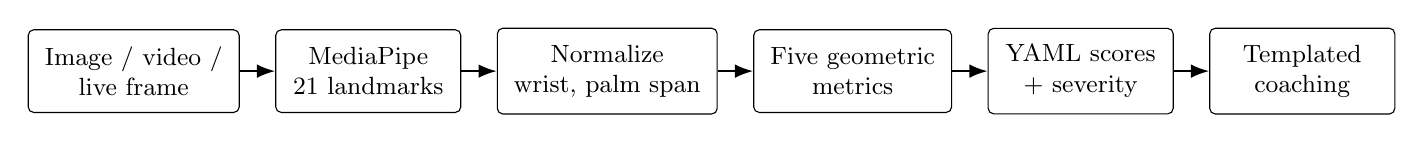
\begin{tikzpicture}[
  font=\small,
  box/.style={draw, rounded corners=2pt, align=center, inner sep=6pt, minimum height=1.05cm, minimum width=2.35cm},
  arr/.style={-{Latex}, thick}
]
\node[box] (in) {Image / video /\\live frame};
\node[box, right=0.45cm of in] (mp) {MediaPipe\\21 landmarks};
\node[box, right=0.45cm of mp] (n) {Normalize\\wrist, palm span};
\node[box, right=0.45cm of n] (f) {Five geometric\\metrics};
\node[box, right=0.45cm of f] (s) {YAML scores\\+ severity};
\node[box, right=0.45cm of s] (c) {Templated\\coaching};
\draw[arr] (in) -- (mp);
\draw[arr] (mp) -- (n);
\draw[arr] (n) -- (f);
\draw[arr] (f) -- (s);
\draw[arr] (s) -- (c);
\end{tikzpicture}%
}
\caption{The core pipeline. Every product surface---photo, video, live, batch---runs this chain. Live mode can run MediaPipe in the browser and enter the chain at landmarks.}
\label{fig:pipeline}
\end{figure}

%----------------------------------------------------------------------
\section{Scoring theory: from a metric to a number a student can use}
\label{sec:scoring}
%----------------------------------------------------------------------

A raw angle is not coaching.
Students need a 0--100 score, a severity word, and a next action.
The mapping is a piecewise-linear \enquote{good in the middle} function defined in YAML so it can be tuned without code changes.

For each criterion, configuration supplies an ideal interval \([I_L, I_H]\) (score 100) and a limit interval \([L_L, L_H]\) (score 0 at or beyond the edges).
If \(x\) is the raw metric,
\begin{equation}
  \operatorname{score}(x) =
  \begin{cases}
    0, & x \le L_L \text{ or } x \ge L_H, \\[0.3em]
    100, & I_L \le x \le I_H, \\[0.3em]
    100 \cdot \dfrac{x - L_L}{I_L - L_L}, & L_L < x < I_L, \\[0.3em]
    100 \cdot \dfrac{L_H - x}{L_H - I_H}, & I_H < x < L_H.
  \end{cases}
\end{equation}
Inside the ideal band the score is a plateau at 100.
Outside, it falls linearly to zero at the limit.
That shape is the geometric cousin of a membership function: healthy technique is a \emph{range}, not a single target angle.

Severity is a second, coarser map:
\begin{equation}
  \operatorname{severity}(s) =
  \begin{cases}
    \text{good}, & s \ge 80, \\
    \text{warning}, & s \ge 50, \\
    \text{critical}, & s < 50.
  \end{cases}
\end{equation}

The composite score is
\begin{equation}
  C = \frac{\sum_k w_k s_k}{\sum_{k:s_k \text{ finite}} w_k},
\end{equation}
with default weights \(w\) as in Section~3.

Thresholds were originally pedagogical guesses.
On 19~September 2026 they were recalibrated from \code{notebooks/scoring\_tuning.ipynb} on \emph{train files only}, and promoted because hold-out macro accuracy rose from 0.622 to 0.689 (Cohen's \(\kappa\) from 0.064 to 0.103).
That is real progress and still far from the 85\% agreement target.
The notebook is forbidden from auto-writing YAML: promotion is a human gate so test-set peeking cannot silently become production~\cite{mlupgrade}.

%----------------------------------------------------------------------
\section{Coaching: language without a language model}
\label{sec:coaching}
%----------------------------------------------------------------------

Scoring says \emph{how wrong}.
Coaching says \emph{what to do}.
The two files are deliberately separate: \code{scoring.yaml} is math; \code{coaching.yaml} is copy.

For every non-good criterion the engine emits a tip with a problem sentence and a fix sentence.
Direction is computed from the same ideal band used for scoring:
\texttt{too\_low} if the metric is below \(I_L\), \texttt{too\_high} if above \(I_H\), otherwise a generic fallback.
That is why \enquote{your wrist is dropping} and \enquote{your wrist is too high} are different templates, not one vague warning.

Tips are ranked so critical issues outrank warnings.
The primary tip is highlighted on the overlay using a small landmark subset for that criterion---wrist and MCPs for height and arch, the long-finger chain for curvature, thumb and index for thumb position.
If every criterion is good, the student sees a single encouragement line rather than five green lectures.

I chose templates over an LLM for v1 after writing it down as an open question in the PRD~\cite{prd}.
The reasons were practical:

\begin{itemize}
  \item Live scoring is throttled to about 2--4~Hz. An LLM round-trip per frame is latency, cost, and jitter.
  \item Coaching has to be unit-testable. A template catalog has a right answer; a chat model does not.
  \item The tone has to stay encouraging and non-judgmental for beginners and children. YAML can be edited; a prompt is a moving target.
\end{itemize}

An LLM may later \emph{rewrite} structured tips into friendlier prose.
It should not be the thing that decides whether a wrist is collapsed.

%----------------------------------------------------------------------
\section{How the software is put together}
\label{sec:arch}
%----------------------------------------------------------------------

\subsection{One engine, four doors}

The important architectural decision was to stop forking the pipeline every time a new UI appeared.
Detection, geometry, scoring, coaching, and overlay live in \code{src/technique\_titan/}.
Everything else is a door into that library.

\begin{figure}[ht]
\centering
\resizebox{\textwidth}{!}{%
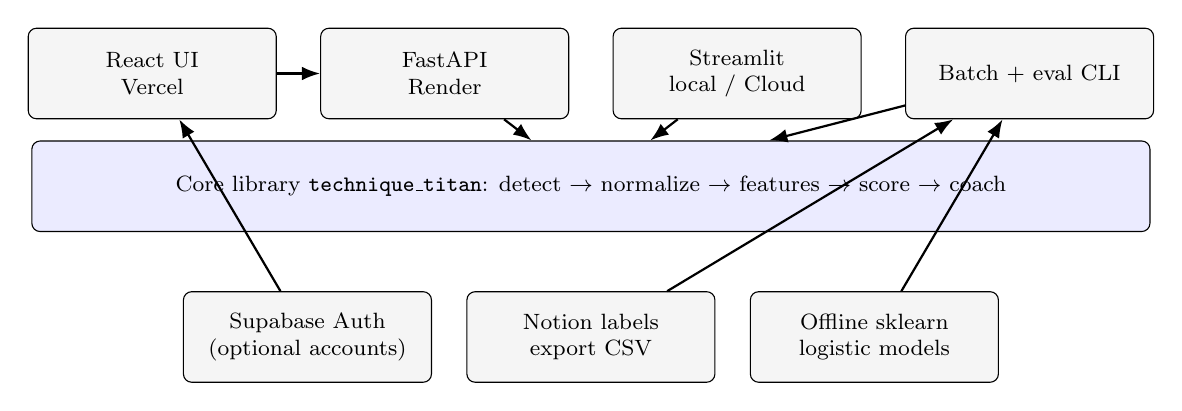
\begin{tikzpicture}[
  font=\footnotesize,
  layer/.style={draw, rounded corners=3pt, align=center, inner sep=7pt, minimum width=3.15cm, minimum height=1.15cm},
  core/.style={layer, fill=blue!8},
  door/.style={layer, fill=gray!8},
  arr/.style={-{Latex}, thick}
]
\node[door] (web) {React UI\\Vercel};
\node[door, right=0.55cm of web] (api) {FastAPI\\Render};
\node[door, right=0.55cm of api] (st) {Streamlit\\local / Cloud};
\node[door, right=0.55cm of st] (cli) {Batch + eval CLI};
\node[core, below=0.85cm of $(web)!0.5!(cli)$, minimum width=14.2cm] (lib) {Core library \texttt{technique\_titan}: detect \(\to\) normalize \(\to\) features \(\to\) score \(\to\) coach};
\node[door, below=0.75cm of lib, xshift=-3.6cm] (sb) {Supabase Auth\\(optional accounts)};
\node[door, below=0.75cm of lib] (no) {Notion labels\\export CSV};
\node[door, below=0.75cm of lib, xshift=3.6cm] (ml) {Offline sklearn\\logistic models};
\draw[arr] (web) -- (api);
\draw[arr] (api) -- (lib);
\draw[arr] (st) -- (lib);
\draw[arr] (cli) -- (lib);
\draw[arr] (no) -- (cli);
\draw[arr] (ml) -- (cli);
\draw[arr] (sb) -- (web);
\end{tikzpicture}%
}
\caption{Product surfaces share one engine. Auth never sits on the analyze path. Offline ML trains from batch exports and is not wired into the API.}
\label{fig:arch}
\end{figure}

\paragraph{Core library.}
\code{detection/hand\_detector.py} wraps MediaPipe.
\code{geometry/} holds vectors, angles, normalization, and plane fits.
\code{features/} implements the five criteria.
\code{scoring.py} and \code{coaching.py} apply YAML.
\code{analysis.py} is the shared single-frame entry point used by Streamlit, the API, and overlays: detect, resolve labels, extract, score, draw.

\paragraph{Batch CLI.}
\code{python -m technique\_titan.batch.process\_folder} walks \code{data/raw/}, writes per-hand CSV and JSON, and flags outliers.
This is how a folder of practice photos becomes a table a notebook can plot.

\paragraph{Eval CLI.}
\code{python -m technique\_titan.eval} merges that table with expert labels, respects a frozen hold-out split, and reports per-criterion accuracy, Cohen's \(\kappa\), and confusion matrices.

\paragraph{Streamlit.}
\code{app.py} at the repo root is the interim research UI: photo, video, local live camera.
It remains useful.
It is no longer the public product.

\paragraph{FastAPI.}
\code{api/} exposes analyze endpoints, public config, health, CORS, and tiered rate limits.
MediaPipe is loaded lazily so \code{GET /v1/health} can pass a Render deploy check without waiting on the Hands graph.

\paragraph{React.}
\code{web/} is the product: marketing home, photo, video, live, about, optional login/signup, owner admin.
It is TypeScript, Vite, Tailwind.
Production is Vercel with root directory \code{web}.

\subsection{The API contract}

\begin{table}[ht]
\centering
\caption{Public API surface. Analyze stays unauthenticated.}
\label{tab:api}
\begin{tabularx}{\textwidth}{@{}ll>{\raggedright\arraybackslash}X@{}}
\toprule
\textbf{Method} & \textbf{Path} & \textbf{Role} \\
\midrule
POST & \code{/v1/analyze/image} & Photo, max 8~MB JPEG/PNG \\
POST & \code{/v1/analyze/frame} & Live JPEG fallback, same contract \\
POST & \code{/v1/analyze/video} & Video, max 40~MB, stride and max-frame caps \\
POST & \code{/v1/score/landmarks} & Score browser-extracted landmarks (up to two hands) \\
GET & \code{/v1/health} & Deploy and status banner \\
GET & \code{/v1/config/public} & Criterion labels and supported modes \\
\bottomrule
\end{tabularx}
\end{table}

Rate limits are path-tiered because live landmarks arrive at a few hertz while photo uploads do not.
Defaults are 360 landmark posts, 120 frames, and 60 image/video uploads per minute window.
A single flat 60 POST/min budget made live practice die with HTTP 429 after about fifteen seconds~\cite{errors}.
That bug taught a product lesson: a posture coach that scolds you for using it in real time is not a coach.

\subsection{Live mode is two different programs}

Hosted live camera cannot be \code{cv2.VideoCapture(0)} on a server.
The server has no webcam.
Streamlit Cloud taught that the hard way~\cite{errors}.

The React live page therefore prefers on-device detection:

\begin{enumerate}
  \item \code{@mediapipe/tasks-vision} runs in the browser, draws the skeleton immediately, and posts compact landmarks to \code{/v1/score/landmarks}.
  \item Video never leaves the device on that path. That is also the privacy story (NFR-SEC-2).
  \item Frame-upload mode still exists as a fallback: canvas JPEGs to \code{/v1/analyze/frame}.
\end{enumerate}

Score updates are throttled; the preview can run at camera rate.
The canvas holds the last good scores while an API call is in flight, otherwise the overlay flickers every frame~\cite{errors}.

Local Streamlit live is the older path: full \code{opencv-python} (not headless), AVFoundation on macOS, and OpenCV capture.
Headless OpenCV is correct for Docker and Cloud and cannot open a Mac camera.
Those two OpenCV packages must never share one resolver.

%----------------------------------------------------------------------
\section{The journey: what was built, and when}
\label{sec:timeline}
%----------------------------------------------------------------------

Technique Titan did not appear as a React app.
It accumulated, sometimes in bursts of a single day, around a problem I already understood from the bench.

\subsection{2024 --- a hand-tracking sketch}

On 17~September 2024 I uploaded a tiny Computer Vision experiment: \code{HandTrackingMin.py}, \code{HandTrackingModule.py}, and a progress document.
It was the first proof that MediaPipe could see a hand on my machine.
It was not yet a piano product.
The later error log still remembers a syntax issue in that legacy module; the modern code lives under \code{src/technique\_titan/}, not those copies~\cite{errors}.

Then the project went quiet.

\subsection{June 2026 --- the prototype comes back}

Around 15~June 2026 the work restarted as an OpenCV and MediaPipe webcam demo.
Two failures defined that week.
MediaPipe was missing, then a newer MediaPipe broke \code{mp.solutions}.
macOS denied the camera, empty frames crashed \code{cvtColor}, and it looked like a model bug until the operating system permission dialog was the real answer~\cite{errors}.

That is the true beginning of Technique Titan as a practice tool: a camera, a skeleton, and the realization that the skeleton was not enough without piano-specific geometry.

\subsection{10 July 2026 --- the engine becomes a project}

10~July 2026 is the day the repository became a product codebase rather than a script folder.
A bulk geometry pipeline landed.
Remote history was merged so the 2024 prototype was not erased.
The tree was reorganized into \code{src/}, \code{tests/}, \code{config/}, \code{data/}.
A Streamlit UI appeared.
Two-hand support and Streamlit Cloud config followed the same day.

So did a pile of environment damage.
A virtualenv still pointed at a removed Python 3.9.
A fresh install pulled MediaPipe 0.10.35.
Streamlit Cloud tried Python 3.13, mixed GUI and headless OpenCV, and lacked \code{libgl1}.
Local live camera then broke because Cloud's headless pin cannot talk to AVFoundation~\cite{errors}.

By night the shape of the next year was already visible: pin the stack, keep Cloud and laptop OpenCV different, and never assume the server can see the user's webcam.

\subsection{Late July 2026 --- coaching, then a real frontend}

On 23~July the feedback engine landed: YAML coaching, compressed so live practice could keep the camera and the primary tip co-visible.
That co-visibility rule still governs the React live layout.

On 28--30~July the public face changed.
A cinematic React UI replaced the idea that Streamlit would be the product.
Landing-page media, icons, theme tokens, Vite proxying, and API rate limits were all learned under time pressure.
\code{npm install} at the repo root does nothing useful; the frontend lives in \code{web/}.
A missing \code{VITE} proxy to port 8000 is a 502 the moment a hand appears, because no-hand frames never hit the API~\cite{errors}.

This was the moment Technique Titan became something I could send to a person who does not own a Python environment.

\subsection{August 2026 --- documentation, deploy, and data}

Early August wrote the PRD, the about page, and the error log as a first-class document---unusual for a student project, and now mandatory reading before any new work~\cite{errors}.
Scoring was fine-tuned by hand.

Deploy was a second education.
The API went to Railway; the UI to Vercel.
Opening the API root URL returns \texttt{Not Found}, which is correct and confusing.
Missing \code{VITE\_API\_BASE\_URL} made the browser POST to Vercel itself and fail with 405.
Vite bakes environment variables at build time, so changing them without a redeploy does nothing.

On 17~August Railway's service disappeared with the subscription.
Production showed \enquote{Load failed}.
The API moved to Render, with CORS limited to the Vercel origin and forwarded-IP trust enabled so rate limits see the real client behind the proxy~\cite{deploy}.

On 24--25~August the research loop started to look like research.
A classification table in Notion became the ground-truth store.
The first labeled dataset landed.
Batch export and normalization produced \code{batch\_summary.csv}.
macOS's case-insensitive disk hid camelCase files that would fail Linux CI; those paths were renamed in two-step \code{git mv}s~\cite{errors}.

\subsection{September 2026 --- video, evaluation, accounts, and ML}

The first half of September was product craft: restyled score panels, video landmark replay, landing clips, and an evaluation harness with a frozen hold-out split.

On 17~September optional accounts shipped: email and Google via a dedicated Supabase project.
Analyze routes stayed public.
An owner \code{/admin} page lists signups.
Auth then failed in the ways hosted auth always fails: truncated JWT keys, Site URL left at \code{localhost:3000}, Google users missing from \code{profiles}, admin checks reading an email claim Google tokens often omit~\cite{errors}.
Each of those is now a checklist item, not folklore.

On 18~September an offline classical ML loop landed: per-criterion L2 logistic regression, joblib artifacts, a compare mode in eval~\cite{mllogistic}.
Production still uses YAML.

On 19~September laterality was inverted for unmirrored photos, which unblocked honest evaluation, and calibrated scoring bands were promoted from the tuning notebook.

Table~\ref{tab:timeline} is the compressed chronology.

\begin{table}[ht]
\centering
\caption{Build timeline, from git history and the error log.}
\label{tab:timeline}
\begin{tabularx}{\textwidth}{@{}l>{\raggedright\arraybackslash}X@{}}
\toprule
\textbf{When} & \textbf{What was built} \\
\midrule
Sep 2024 & First MediaPipe hand-tracking scripts. \\
Jun 2026 & Webcam prototype; camera permissions; MediaPipe pin. \\
10 Jul 2026 & Geometry engine, package layout, Streamlit, two-hand, Cloud. \\
23 Jul 2026 & Templated coaching; compact live feedback. \\
28--30 Jul 2026 & React product UI, FastAPI live path, rate limits, CORS. \\
5--8 Aug 2026 & PRD, about page, error log, scoring edits, first hosted API. \\
17 Aug 2026 & API host: Railway \(\to\) Render. \\
24--25 Aug 2026 & Notion labels, first dataset, batch CSV. \\
2--11 Sep 2026 & Video replay, landing media, eval harness. \\
17 Sep 2026 & Supabase email/Google auth and admin stats. \\
18 Sep 2026 & Offline logistic scoring loop. \\
19 Sep 2026 & Anatomical laterality; calibrated YAML thresholds. \\
\bottomrule
\end{tabularx}
\end{table}

Roadmap status as of this writing~\cite{roadmap}: Phases 0, 1, 2, and 3a are done.
Phase 3b accounts are done; session persistence and progress charts are not.
Phase 4 intelligence is underway as eval plus offline ML, not as a custom detector.
Phase 5 (performance, accessibility audit, monetization) is planned.

%----------------------------------------------------------------------
\section{Product surfaces: what a user actually touches}
\label{sec:product}
%----------------------------------------------------------------------

\subsection{Marketing and orientation}

The home page is cinematic on purpose.
Piano posture is a visual craft; the site should feel like a studio, not a dashboard demo.
An about page states the origin story in the same words I would tell a teacher: most practice happens alone, and Technique Titan is a second pair of eyes.

\subsection{Photo, video, live}

Photo is the simplest honest loop: one still, one overlay, five scores, ranked tips.
Video adds time.
The API samples frames with a stride and a max-frame cap so a four-minute practice film cannot become an unbounded MediaPipe job.
The React video page replays landmarks and charts scores so a collapsed wrist is a dip on a timeline, not a forgotten moment.

Live is the mode I actually wanted at the piano.
It is also the mode that forced the most architecture.
Browser MediaPipe keeps the preview fluid.
The API scores landmarks rather than video.
The UI must never hide the camera behind the advice, and must never hide the right hand behind the left.

\subsection{Accounts without locking the coach}

Sign-in is optional.
Photo, video, and live work without an account.
That was a product decision, not a missing feature: a posture check should not require a password.
Supabase holds email and Google identities.
\code{ProtectedRoute} exists so analyze can be gated later.
Owner admin lists \code{auth.users} rather than hoping a profiles trigger already ran.

What accounts do \emph{not} yet do is remember yesterday's session.
Progress charts are the next product slice (Phase 3b remainder).
Until then, the \enquote{journey} a student can see is one sitting, not a semester.

%----------------------------------------------------------------------
\section{Data, labels, and evaluation}
\label{sec:eval}
%----------------------------------------------------------------------

\subsection{A small, serious dataset}

Raw images live under \code{data/raw/} in severity folders: \code{excellent/}, \code{good/}, \code{warning/}, \code{critical/}, with numbered filenames.
They are gitignored.
Ground truth does not live in git either.
It lives in a Notion classification table titled \code{techniquetitan}.
Columns are filename, hand, the five criteria, and notes~\cite{datareadme}.
Export to \code{data/labels.csv} is what the batch and eval CLIs consume.

Each criterion is labeled independently as good, warning, or critical, plus left/right (or both).
That matches how a teacher actually talks: a hand can have a beautiful arch and a terrible wrist.

Additional \code{f*} paths have labels without requiring extra photographs; their geometry lives in \code{data/synthetic/feature\_rows.csv} so the offline trainer can run without another MediaPipe batch.

\subsection{The evaluation contract}

Accuracy talk without a frozen split is just overfitting with extra steps.
The harness therefore:

\begin{enumerate}
  \item Merges predictions to labels in a \emph{hand-aware} way (\code{left}/\code{right} versus \code{both}). The batch CSV still joins labels by filename only; eval is stricter.
  \item Tags train versus hold-out using \code{data/eval/holdout\_split.json}, split by filename and stratified by severity folder.
  \item Reports per-criterion accuracy, Cohen's \(\kappa\), and confusion matrices.
\end{enumerate}

Cohen's \(\kappa\) matters because a model that always says \texttt{good} can look accurate on a set that is mostly good.
\(\kappa\) asks whether agreement exceeds chance.

CI runs eval \emph{unit tests}, not a MediaPipe pass over \code{data/raw/}.
A full agreement report is a local artifact under \code{data/eval/reports/}, which is gitignored.
There is no in-repo hold-out number that meets the 85\% bar.
After the 19~September calibration, hold-out macro accuracy was 0.689.
That is the honest headline.

\subsection{What evaluation already changed}

Two scientific bugs were invisible until eval existed.
Laterality mismatch made the hold-out set look tiny and random.
YAML bands that \enquote{looked right} on the images I stared at did not maximize hold-out agreement.
The loop---label, batch, eval, notebook on train, promote only if hold-out rises---is the actual ML project.
A new architecture is not.

%----------------------------------------------------------------------
\section{Offline machine learning: learning teacher judgment, not a new eye}
\label{sec:ml}
%----------------------------------------------------------------------

\subsection{The mapping we actually want to learn}

Let \(\mathbf{x}\) be a feature vector built from geometry, and let \(y \in \{\text{good},\text{warning},\text{critical}\}\) be an expert label for one criterion.
Production heuristics map one scalar metric through YAML, then bucket the 0--100 score.
Multinomial logistic regression learns
\begin{equation}
  P(y=c\mid\mathbf{x}) = \frac{\exp(\mathbf{w}_c\cdot\mathbf{x}+b_c)}{\sum_{c'}\exp(\mathbf{w}_{c'}\cdot\mathbf{x}+b_{c'})}.
\end{equation}
The predicted class is \(\arg\max_c P(y=c\mid\mathbf{x})\).
Training minimizes cross-entropy on the train split with L2 regularization and balanced class weights, after median imputation and standard scaling~\cite{mllogistic}.

There are five separate classifiers, not one multi-label net.
Wrist height and thumb position have different drivers.
A hand can be good on arch and critical on lateral deviation.
Small \(N\) makes a joint model hungry.
Per-criterion weights stay inspectable.

\subsection{Why the feature vector is not \enquote{the one YAML number}}

A linear model on a single metric cannot represent \enquote{good in the middle.}
If healthy wrist height is a band, a straight line in that one variable cannot make both \enquote{too low} and \enquote{too high} look like the same bad class without help.

So \(\mathbf{x}\) includes the raw geometry (\(\sim\)20 numeric columns: deltas, joint angles, arch ratio, confidence, \ldots), plus derived terms
\begin{align}
  \text{outside} &= \max(0, I_L-x) + \max(0, x-I_H), \\
  \text{outside}^2, &\quad \lvert x - \text{center}\rvert,
\end{align}
and a left/right one-hot.
Those extras make two-sided YAML bands linearly representable, and they let the model use more than one measurement at a time---for example wrist height together with arch and detection confidence.

The model never sees pixels.
It never sees the heuristic score or the label columns inside \(\mathbf{x}\).

\subsection{What this does and does not mean}

It means the project has a data-calibrated alternative to hand-tuned 1-D bands, evaluated on the same frozen split.
It does not mean production is \enquote{an ML app} now.
The API still serves YAML.
Wiring \code{ml\_with\_fallback} is a follow-up slice, and heuristics remain the documented fallback~\cite{prd,mlupgrade}.

The upgrade path after that is also sequenced on purpose:

\begin{enumerate}
  \item Keep measuring heuristic versus ML agreement.
  \item Add a viewpoint / quality rejector so top-down shots are not scored as confident technique errors.
  \item Add temporal habits: smoothing, dwell, session-level patterns. Today every frame is independent, which is not how a collapsed wrist actually lives.
  \item Only later, piano-specific vision: key plane, Pose/Holistic forearm, so wrist height is versus the keyboard rather than versus knuckles, and lateral deviation uses a real forearm line.
\end{enumerate}

What we are not doing yet: fine-tuning Hands on thirty photos, training a pixel-to-score CNN, or using an LLM as a scorer.

%----------------------------------------------------------------------
\section{Deployment, privacy, and the production texture of the project}
\label{sec:deploy}
%----------------------------------------------------------------------

\subsection{Where the pieces run}

\begin{table}[ht]
\centering
\caption{Production topology.}
\label{tab:deploy}
\begin{tabularx}{\textwidth}{@{}ll>{\raggedright\arraybackslash}X@{}}
\toprule
\textbf{Surface} & \textbf{Host} & \textbf{Notes} \\
\midrule
React UI & Vercel & Root directory \code{web}; env baked at build \\
API & Render (Docker) & Free tier cold start \(\sim\)30--60~s after idle \\
Accounts & Supabase & Dedicated project; anon key only on the frontend \\
Interim demo & Streamlit Cloud & Photo/video; no hosted live camera \\
\bottomrule
\end{tabularx}
\end{table}

CORS must list the Vercel origin.
Wildcard CORS cannot be paired with credentials.
Trusting \code{X-Forwarded-For} is gated on \code{TRUST\_PROXY}, because a client could otherwise spoof an IP and evade rate limits~\cite{errors,deploy}.

\subsection{Privacy}

Uploaded media is processed in request scope.
There is no account-linked store of practice videos yet, which is both a privacy win and the reason progress tracking does not exist.
Live landmarks mode sends numbers, not pixels.
That is the design I want at the piano: the coach sees a skeleton, not a recording of my living room.

\subsection{CI and reproducibility}

GitHub Actions runs pytest on Python 3.11 and \code{npm run build} on Node 22.
Tests cover geometry fixtures, scoring, coaching, analysis, API, eval units, and ML training smoke.
The error log is part of the engineering process: agents and future-me are required to read it before changing the stack, so we do not reintroduce a fixed failure mode~\cite{errors}.

%----------------------------------------------------------------------
\section{Hard-won lessons: how the pieces learned to fit}
\label{sec:lessons}
%----------------------------------------------------------------------

A timeline of features is incomplete without the constraints those features discovered.
A few patterns repeated until they became architecture.

\paragraph{The stack is a single organism.}
MediaPipe 0.10.21, NumPy 1.x, OpenCV 4.10, Python 3.11.
Unpin one and the others fail in a different environment---laptop, Cloud, Docker, CI.

\paragraph{Where the camera lives decides the product.}
Local OpenCV capture, Cloud Streamlit, and browser MediaPipe are three different machines.
Hosted live belongs in the browser.

\paragraph{Configuration is a product surface.}
Thresholds, copy, CORS, rate limits, and auth URLs are all \enquote{just config} until they silently ship the wrong behavior.
YAML for scoring and coaching was the right instinct; Vite bake-time env vars need the same respect.

\paragraph{UX for two hands is a layout problem, not a model problem.}
If the right-hand card is below the fold, the detector may as well have returned one hand.

\paragraph{Labels are part of the codepath.}
Notion, CSV export, laterality conventions, and a frozen split are as load-bearing as \code{scoring.py}.
Until laterality was inverted, eval was measuring the mirror, not the pianist.

\paragraph{Write the failures down.}
\code{docs/errors.md} is chronological on purpose.
E01 through E34 are not a shame log.
They are the reason the next change is cheaper.

%----------------------------------------------------------------------
\section{How the pieces come together today}
\label{sec:together}
%----------------------------------------------------------------------

If I sit at a piano and open the live page, this is the path:

The browser asks for the camera.
MediaPipe Tasks draws 21 points on a mirrored canvas.
Every so often a compact landmark payload crosses the network to Render.
FastAPI does not run Hands again.
It normalizes, extracts five metrics, applies \code{scoring.yaml}, selects tips from \code{coaching.yaml}, and returns scores.
The React canvas keeps the last good result so the skeleton does not blink.
I see a color, a composite, and one sentence to change.

If I instead upload a photo of a student's hands, MediaPipe runs on the server, laterality is inverted to anatomical labels, both hands are scored, and an overlay PNG comes back.

If I am tuning the engine, I drop images into \code{data/raw/}, export Notion to \code{data/labels.csv}, run batch, run eval, open the notebook, and refuse to touch YAML unless hold-out improves.
I can train five logistic models into \code{config/models/} and compare them to heuristics without putting them on Vercel.

If I am deploying, Vercel serves the SPA, Render serves Dockerized Uvicorn, Supabase serves optional identity, and Streamlit Cloud remains a research side door.

Those are not separate apps that happen to share a name.
They are one measurement idea---normalized hand geometry scored like a teacher talks---with several I/O adapters.
The adapters were built in the order pain arrived: scripts, then a library, then Streamlit, then an API, then React, then labels, then eval, then auth, then offline ML.
Each adapter made the next one possible.
None of them replaced the engine.

The remaining seams are equally clear.
Persistence will turn a sitting into a history.
A viewpoint gate will stop scoring the wrong camera angle with false confidence.
A forearm and key-plane model will make two of the five metrics physically truer.
A learned scorer will ship only when it beats YAML on hold-out with the heuristic still behind it.
Teacher accounts will matter after there is something worth assigning.

That is what \enquote{coming together} means here.
Not that the project is finished.
That the parts finally share a spine.

%----------------------------------------------------------------------
\section{Limitations and next work}
\label{sec:next}
%----------------------------------------------------------------------

The honest limitations are documented in the ML upgrade note and the PRD, and they are still true~\cite{mlupgrade,prd}.

\begin{itemize}
  \item Wrist lateral deviation uses MCP axes as a forearm proxy.
  \item Wrist height is versus knuckles, not versus the keyboard.
  \item Viewpoint is not gated.
  \item Frames are independent; habits are temporal.
  \item Expert agreement is below the 85\% target on hold-out.
  \item The labeled real-image set is small.
  \item Session history, WCAG audit, teacher roles, and monetization are unbuilt.
\end{itemize}

The next construction sequence is the one the roadmap already states: persist sessions and draw progress; grow labels; promote ML only with evidence; then piano-specific perception; then scale.
I am more interested in that discipline than in a dramatic rewrite.

%----------------------------------------------------------------------
\section{Conclusion}
%----------------------------------------------------------------------

Technique Titan began as a curiosity: can a camera see a hand well enough to talk about piano technique?
It became a geometry engine, then a coach, then a website, then a hosted product, then an evaluation loop, then an offline model that still does not get to talk to users until it earns it.

The concepts underneath are classical on purpose.
Landmarks, invariance, joint angles, planes, piecewise maps, templates, hold-out splits, logistic regression.
The journey was not classical: permission dialogs, pin conflicts, Cloud versus laptop OpenCV, Vercel talking to a dead Railway domain, Google JWTs without email, a detector that thinks in mirrors.

What holds it together is a single sentence I would still write on a whiteboard.
Detect a hand.
Measure the shapes a teacher already names.
Score them the same way every time.
Say the next correction in language a beginner can use.
Then measure whether a teacher would have said the same thing.

That loop is the product.
The rest is plumbing---necessary, hard-won, and finally pointed in the same direction.

%----------------------------------------------------------------------
\appendix
\section{Landmark index reference}
%----------------------------------------------------------------------

MediaPipe Hands indices used throughout the engine:

\begin{center}
\begin{tabular}{cl}
\toprule
\textbf{Index} & \textbf{Name} \\
\midrule
0 & Wrist \\
1--4 & Thumb CMC, MCP, IP, TIP \\
5--8 & Index MCP, PIP, DIP, TIP \\
9--12 & Middle MCP, PIP, DIP, TIP \\
13--16 & Ring MCP, PIP, DIP, TIP \\
17--20 & Pinky MCP, PIP, DIP, TIP \\
\bottomrule
\end{tabular}
\end{center}

\section{Local development sketch}

The product stack is two processes.
Python 3.11 virtualenv with \code{pip install -e ".[api]"}, then \code{uvicorn api.main:app --reload --port 8000}.
In \code{web/}, \code{npm install} and \code{npm run dev}.
Vite proxies \code{/v1/*} to port 8000.
Optional auth uses \code{web/.env.local} with \code{VITE\_SUPABASE\_URL} and \code{VITE\_SUPABASE\_ANON\_KEY} from the same Supabase project.

Batch and eval must use that virtualenv, not Homebrew \code{python3.11}, which does not have the editable package~\cite{errors}.

\section{Selected repository map}

\begin{verbatim}
api/                     FastAPI backend
web/                     React + TypeScript product UI
src/technique_titan/     detect, geometry, features, score, coach
config/scoring.yaml      piecewise-linear thresholds
config/coaching.yaml     tip catalog
data/raw/                labeled images (gitignored)
data/eval/holdout_split.json
notebooks/scoring_tuning.ipynb
supabase/                auth schema and migrations
docs/PRD.md, ROADMAP.md, errors.md
\end{verbatim}

\begin{thebibliography}{99}

\bibitem{prd}
A.~Dutta, \enquote{Technique Titan --- Product Requirements Document,} in-repo \texttt{docs/PRD.md}, draft v1.1, 5~Aug~2026.

\bibitem{roadmap}
A.~Dutta, \enquote{Technique Titan --- Roadmap,} in-repo \texttt{docs/ROADMAP.md}, draft v1.1, 11~Sep~2026.

\bibitem{scoringmethods}
A.~Dutta, \enquote{Scoring Methods,} in-repo \texttt{docs/SCORING\_METHODS.md}, 5~Aug~2026.

\bibitem{mlupgrade}
A.~Dutta, \enquote{Technique Titan --- ML Upgrade Path,} in-repo \texttt{docs/ML\_UPGRADE.md}, 18~Sep~2026.

\bibitem{mllogistic}
A.~Dutta, \enquote{Offline learned scorer --- multinomial logistic regression,} in-repo \texttt{docs/ML\_LOGISTIC\_REGRESSION.md}, 18~Sep~2026.

\bibitem{deploy}
A.~Dutta, \enquote{Website deployment,} in-repo \texttt{docs/DEPLOY.md}.

\bibitem{errors}
A.~Dutta, \enquote{Technique Titan --- Error History,} in-repo \texttt{docs/errors.md}, entries E01--E34, Jun--Sep~2026.

\bibitem{datareadme}
A.~Dutta, \enquote{Data intake,} in-repo \texttt{data/README.md}.

\bibitem{mediapipe}
Google, \enquote{MediaPipe Hands / Hand Landmarker,} \url{https://ai.google.dev/edge/mediapipe/solutions/vision/hand_landmarker}.

\bibitem{opencv}
OpenCV team, \enquote{OpenCV Library,} \url{https://opencv.org/}.

\bibitem{fastapi}
S.~Ram\'irez, \enquote{FastAPI,} \url{https://fastapi.tiangolo.com/}.

\bibitem{react}
Meta, \enquote{React,} \url{https://react.dev/}.

\bibitem{sklearn}
F.~Pedregosa et~al., \enquote{Scikit-learn: Machine Learning in Python,} \textit{JMLR}, 12:2825--2830, 2011.

\end{thebibliography}

\end{document}
